
%%%%%%%%%%%%%%%%%%%%%%%%%%%%%%%%%%%%%%%%%%%%%%%%%%%%%%%%%%%%%%%%%%%%%
%% This is a (brief) model paper using the achemso class
%% The document class accepts keyval options, which should include
%% the target journal and optionally the manuscript type.
%%%%%%%%%%%%%%%%%%%%%%%%%%%%%%%%%%%%%%%%%%%%%%%%%%%%%%%%%%%%%%%%%%%%%
\documentclass[journal=ancham,manuscript=article]{achemso}

%%%%%%%%%%%%%%%%%%%%%%%%%%%%%%%%%%%%%%%%%%%%%%%%%%%%%%%%%%%%%%%%%%%%%
%% Place any additional packages needed here.  Only include packages
%% which are essential, to avoid problems later.
%%%%%%%%%%%%%%%%%%%%%%%%%%%%%%%%%%%%%%%%%%%%%%%%%%%%%%%%%%%%%%%%%%%%%
\usepackage{chemformula} % Formula subscripts using \ch{}
\usepackage{achemso}
\usepackage[T1]{fontenc} % Use modern font encodings
\usepackage{amsmath}
\usepackage{subfigure}
\usepackage{amsfonts}
\usepackage{multirow}

%%%%%%%%%%%%%%%%%%%%%%%%%%%%%%%%%%%%%%%%%%%%%%%%%%%%%%%%%%%%%%%%%%%%%
%% If issues arise when submitting your manuscript, you may want to
%% un-comment the next line.  This provides information on the
%% version of every file you have used.
%%%%%%%%%%%%%%%%%%%%%%%%%%%%%%%%%%%%%%%%%%%%%%%%%%%%%%%%%%%%%%%%%%%%%
%%\listfiles

%%%%%%%%%%%%%%%%%%%%%%%%%%%%%%%%%%%%%%%%%%%%%%%%%%%%%%%%%%%%%%%%%%%%%
%% Place any additional macros here.  Please use \newcommand* where
%% possible, and avoid layout-changing macros (which are not used
%% when typesetting).
%%%%%%%%%%%%%%%%%%%%%%%%%%%%%%%%%%%%%%%%%%%%%%%%%%%%%%%%%%%%%%%%%%%%%
\newcommand*\mycommand[1]{\texttt{\emph{#1}}}

%%%%%%%%%%%%%%%%%%%%%%%%%%%%%%%%%%%%%%%%%%%%%%%%%%%%%%%%%%%%%%%%%%%%%
%% Meta-data block
%% ---------------
%% Each author should be given as a separate \author command.
%%
%% Corresponding authors should have an e-mail given after the author
%% name as an \email command. Phone and fax numbers can be given
%% using \phone and \fax, respectively; this information is optional.
%%
%% The affiliation of authors is given after the authors; each
%% \affiliation command applies to all preceding authors not already
%% assigned an affiliation.
%%
%% The affiliation takes an option argument for the short name.  This
%% will typically be something like "University of Somewhere".
%%
%% The \altaffiliation macro should be used for new address, etc.
%% On the other hand, \alsoaffiliation is used on a per author basis
%% when authors are associated with multiple institutions.
%%%%%%%%%%%%%%%%%%%%%%%%%%%%%%%%%%%%%%%%%%%%%%%%%%%%%%%%%%%%%%%%%%%%%
\author{Valeria Fonseca Diaz}
\email{valeria.fonsecadiaz@kuleuven.be}
\author{Bart De Ketelaere}
\email{bart.deketelaere@kuleuven.be}
\author{Ben Aernouts}
\email{ben.aernouts@gmail.com}
\altaffiliation{Biosystems TC, KU Leuven,
Kleinhoefstraat 4, Geel, Belgium}
\author{Wouter Saeys}
\email{wouter.saeys@kuleuven.be}
\affiliation[KU Leuven]
{KU Leuven, Kasteelpark
Arenberg 30, Leuven, Belgium}
%%%%%%%%%%%%%%%%%%%%%%%%%%%%%%%%%%%%%%%%%%%%%%%%%%%%%%%%%%%%%%%%%%%%%
%% The document title should be given as usual. Some journals require
%% a running title from the author: this should be supplied as an
%% optional argument to \title.
%%%%%%%%%%%%%%%%%%%%%%%%%%%%%%%%%%%%%%%%%%%%%%%%%%%%%%%%%%%%%%%%%%%%%
\title[An \textsf{achemso} demo]
  {On the challenge of unsupervised sample selection for multivariate calibration}

%%%%%%%%%%%%%%%%%%%%%%%%%%%%%%%%%%%%%%%%%%%%%%%%%%%%%%%%%%%%%%%%%%%%%
%% Some journals require a list of abbreviations or keywords to be
%% supplied. These should be set up here, and will be printed after
%% the title and author information, if needed.
%%%%%%%%%%%%%%%%%%%%%%%%%%%%%%%%%%%%%%%%%%%%%%%%%%%%%%%%%%%%%%%%%%%%%
%\abbreviations{IR,NMR,UV}
\keywords{sample selection, multivariate calibration, NIR, PLS}

%%%%%%%%%%%%%%%%%%%%%%%%%%%%%%%%%%%%%%%%%%%%%%%%%%%%%%%%%%%%%%%%%%%%%
%% The manuscript does not need to include \maketitle, which is
%% executed automatically.
%%%%%%%%%%%%%%%%%%%%%%%%%%%%%%%%%%%%%%%%%%%%%%%%%%%%%%%%%%%%%%%%%%%%%

% -----------------------------------------------------
% -------------------BEGIN DOCUMENT ------------
% -----------------------------------------------------

\begin{document}


% -----------------------------------------------------
% ------------------- abstract  ------------
% -----------------------------------------------------
\begin{abstract}
Multivariate calibration models continue to be the most efficient mechanism to indirectly measure chemical compositions based on spectral measurements. The cost of reference analyses for chemical compositions is a major feature of interest to be minimized in industrial applications for the sake of more efficient analytical processes. The present work aims at characterizing the challenge of unsupervised sample selection based on spectral measurements to build calibration models. A scheme to address this challenge in real applications for PLSR models is developed which is defined on the basis of optimal sample size, input dimensionality and selection method.
\end{abstract}%

% -----------------------------------------------------
% ------------------- introduction  ------------
% -----------------------------------------------------

\section{Introduction}\label{introduction}

Multivariate calibration models have been the primary analytical tool to indirectly measure the chemical composition of products making processes such as those of quality control more cost-efficient. Many challenges are still present when building and maintaining these models. The present work presents an exhaustive evaluation of the challenge of unsupervised sample selection to build successful calibration models. Within the range of applications of multivariate calibration, the stated problem is particularly relevant for indirect inspection of collected or observed natural samples using near-infrared (NIR) spectroscopy, as it is the case of the agrofood industry (AFI) \cite{Au2020,Diaz-Olivares2020, Saeys2005, Bobelyn2010}.  

The challenge of unsupervised sample selection relates to determining what the best methodology or strategy is to select the samples that would be worthy of reference analysis (chemical composition values), based on spectral measurements to build calibration models. As it is widely known, spectral measurements are easy and cheap to collect, therefore a vast quantity of units can be submitted to these measurements with low effort. On the contrary, collecting the reference analyses is a task that requires substantial effort, high costs and possibly high waste. This has been the motivation to pay attention to the optimization of model building costs while gaining model building effectiveness. Historically, the interpretation for this gain has been rephrased as the optimal spanning of variability with a minimum number of samples \cite{Naes1990, Saeys2019,Kennard1969}.

Because of the importance of this problem, optimal sample sizes and suitable strategies to select these samples have been active research domains for many years \cite{Ferre1996,Au2020, Liu2019}. Through the last decades, many methods have been proposed for sample selection within a finite set of units, some of them becoming widely accepted for their intuitively accurate approach and good performance \cite{Shetty2012a, Nawar2018, He2015}. The two most popular methods in the context of NIR spectroscopy and multivariate calibration are the Kennard-Stone\cite{Kennard1969} and  Puchwein\cite{Puchwein1988} algorithms. As a strategy, clustering techniques are widely accepted in order to account for multiple sources of variability\cite{Naes1990}, particularly when the collected units groups of samples exist in batches of collected products\cite{Bobelyn2010}. These popular algorithms have the common feature of relying in distance between the samples. Less popular in NIR applications but highly effective in product design are the D-optimal designs of experiments, which translate the concept of variability from distance between samples to the variance of the coefficients of an assumed model \cite{Goos2011}. Yet, no clear understanding exists about which of all these methods are more suitable for NIR applications with multivariate calibration and no exhaustive competition of them has been disseminated to the authors' knowledge. The most recent study found related to this problem used of only the two most popular methods mentioned before \cite{Au2020}.

Multivariate calibration is a concept that in principle can involve any type of statistical model. Moreover, calibrations are made for classification as well as regression tasks. While the present work focuses on regression models, the scheme here presented can serve as guidance for classification models. Regarding the model architecture, as of now, there is little doubt on the effectiveness of the type of bilinear models that are widely used for NIR applications. Unless the spectral values have a strong nonlinear relationship with chemical reference values, bilinear models such as partial least squares regression (PLSR) or principal component regression (PCR) remain the workhorse model architectures. Most of the work that can be found addressing the current problem of interest provides answers about the minimum required sample size using PLSR models \cite{Naes1990, Au2020, Shetty2012a, Rodionova2008}. The diversity on the answers is still large leaving researchers out of the scope for a general answer. 

The present work aims to provide a scheme on how to approach the selection of calibration samples by understanding the properties of PLSR models. The general framework of statistical learning theory by Vapnik provides specific answers on the sample size needed depending on the model architecture to be used\cite{Vapnik2019, Vapnik2000}. To deepen into this question for NIR applications, it is necessary to understand PLSR within the framework explained by Vapnik. In a similar way, to understand the required features to take into account for a successful PLSR model, it is essential to seek for the elements of the PLSR architecture that can be controlled with unsupervised measurements. These aspects are to be described and explained for the state-of-the-art methods to select calibration samples.

A general and a specific framework of PLSR is presented in order to set a context of analysis to solve the problem of the best strategy for unsupervised sample selection. The work is organized as follows. First, a description of the general and specific frameworks is presented prior to the research questions of the current work. Afterwards, the experimental work and results are presented along with the discussion and conclusions about the aspects that lead to a more successful unsupervised sample selection to build calibration models.

% -----------------------------------------------------
% ------------------- frameworks  ------------
% -----------------------------------------------------

\section{Frameworks to understand PLSR}

\subsection{The general framework}

A general framework to understand PLSR models takes place in the context of statistical learning theory. In the general regression task, the response variable is assumed to be a linear combination of basis functions plus an error variable. With that model architecture and using a square loss, the objective to estimate the model is to minimize the square error \cite{Vapnik2019}. More concretely, let $y \in \mathbb{R}$ be the random variable representing the chemical constituent of interest and  $\mathbf{x} \in \mathbb{R}^{p}$ the predictor vector of spectral measurements. The regression model is defined as $ y = f(\mathbf{x}, \boldsymbol{\beta}) + \epsilon$.  The general regression problem with square error can be established as \cite{Vapnik2000}:

\begin{equation}
    \min E \left[ (y-f(\mathbf{x}, \boldsymbol{\beta}))^2\right]; \quad f(\mathbf{x}, \boldsymbol{\beta}) = \sum_{k=1}^{\infty} \beta_k \phi_{k}(\mathbf{x})
    \label{eq_general_regression_problem}
\end{equation}

where $\{\phi_{i}(\mathbf{x})\}$ constitutes a basis of $L_2$ for which its elements can be ordered by some criterion. In the context of statistical learning theory by Vapnik, $E \left[ (y-f(\mathbf{x}, \boldsymbol{\beta}))^2\right]$ is called the \emph{expected risk}, which in practice is replaced by the so-called \emph{empirical risk} in the presence of a set of $n$ observations to estimate function $f$ \cite{Vapnik2000}. This empirical risk is what has been known for centuries as the sum of square errors. The important feature of this optimization task is that to ensure a small \emph{expected risk}, the \emph{empirical risk} is to be minimized only over a limited number of basis functions $\{\phi_{k}(\mathbf{x})\}_{k=1}^d$. Therefore, the regression problem becomes:

\begin{equation}
    \min \frac{1}{n} \sum_{i=1}^n (y_i-f_d(\mathbf{x}_i, \boldsymbol{\beta}))^2; \quad f_d(\mathbf{x}, \boldsymbol{\beta}) = \sum_{k=1}^{d} \beta_k \phi_{k}(\mathbf{x})
    \label{eq_square_loss_empirical_regression_problem}
\end{equation}

It is in this regard that the problem as stated in eq. (\ref{eq_square_loss_empirical_regression_problem}) corresponds to the definition of the PLSR model  \cite{Stone1990}, where the basis $\{\phi_{k}(\mathbf{x})\}$ is constructed by means of maximizing the covariance between $y$ and $\mathbf{x}$. The order in this basis is established by the covariance deflation at each step of the PLSR algorithm. The key element in this framework is the fact that the number of chosen basis functions $d$ corresponds to the so-called $VC$ dimension in Vapnik's theory, which measures the capacity control of a learning machine \cite{Vapnik2019}. The importance of the capacity control parameter $d$ is that it serves as the reference for determining a suitable sample size when aiming to build a regression machine, or, as known in the context of chemometrics, a multivariate calibration model. In the work by Vapnik, it has been stated that the ratio between the sample size and the $VC$ dimension determines whether the sample size is large or small. As the sample becomes large, the empirical risk becomes closer to the expected risk \cite{Vapnik2000}. Although there is no absolute threshold, it is stated that the sample size is considered \emph{large} when  $n/d>20$ \cite{Vapnik2000}.


\subsection{The specific framework}

In the jargon of multivariate calibration, the basis of $L_2$ is what is known as the set of latent variables. Based on a set of $n$ observations stored in the matrices $\mathbf{X}_{n\times p}$ and $Y_{n\times 1}$, the underlying idea of the PLS algorithm is to calculate latent variables $\{\phi_{k}(\mathbf{x})\}$ such that $\phi_k(\mathbf{x}) = \mathbf{Xv}_{k}$, where $\mathbf{v}_k$ results from maximizing the covariance between $\mathbf{X}$ and $Y$ at the $k$-th deflation step \cite{DeJong1993}. 

For a given value of $d$, the set of resulting latent variables constitute a set of orthonormal variables $\{\phi_{k}(\mathbf{x})\}_{i=1}^d$. However, the set of loading vectors $\{\mathbf{v}_k\}$ is regarded as $\mathbf{S}$-orthogonal, i.e. $\mathbf{v}_k'\mathbf{S}\mathbf{v}_j = 0 \quad (j<k)$, where $\mathbf{S}$ is the covariance matrix of $\mathbf{X}$. The $\mathbf{S}$-orthogonality property of the PLSR algorithm clarifies that the estimation of this type of regression model depends highly on the covariance matrix $\mathbf{S}$. This property suggests that if $n<N$ samples are found such that $\mathbf{S}_n$ and $\mathbf{S}_N$ are equivalent, there is no pure unsupervised information discarded that serves the PLSR model in the $N-n$ remaining samples.

There are several methods and indexes to study the equivalence between two matrices \cite{Tomic2013}. For the sake of bilinear regression models such as PLSR, it becomes manifest to evaluate this equivalence via the spectral value decomposition (SVD) of the matrices due to the rank deficiency of $\mathbf{S}$ in NIR applications. The reason is two-fold. On the one hand, two matrices with the same eigenvectors are regarded as congruent matrices which is a type of equivalence relationship\cite{Horn1985}. On the other hand, as the SVD of $\mathbf{S}$ constitutes the theory of principal component analysis (PCA), the eigenvalues of $\mathbf{S}$ account for the variability that the individual dimensions contain and their relative predictive power for a regression model \cite{Artemiou2013}. Thus, the variability explained by two matrices can be compared based on their eigenvalues. Although this comparison directly relates to principal component regression (PCR), the present work focuses on the role of matrix $\mathbf{S}$ for PLSR models.

% -----------------------------------------------------
% ------------------- research questions  ------------
% -----------------------------------------------------

\section{Research questions}

The present work aims at presenting a scheme to approach the problem of unsupervised sample selection for PLSR models models. This scheme is defined in terms of three factors, namely, selection methods, the dimensionality of the matrix $\mathbf{S}$ and sample size to obtain satisfactory performance of calibration models. The objective is to provide the following answers:

\begin{itemize}

    \item Can particular thresholds be found regarding the optimal sample size for satisfactory PLSR models in chemometrics based on the ratio $n/d$?

    \item What is the equivalence achieved between $\mathbf{S}_N$ and $\mathbf{S}_n$ by selection methods, input dimensionality and sample size?
    
    \item What are the most optimal conditions of the three factors for satisfactory PLSR models?

\end{itemize}

% -----------------------------------------------------
% ------------------- experimental  ------------
% -----------------------------------------------------

\section{Experimental}\label{experimental}

\subsection{Case studies}\label{data}

Two AFI real case studies were taken to demonstrate the aspects previously discussed about unsupervised sample selection. Within the availability of real cases, the current ones were chosen to demonstrate the effect of sample selection strategies for chemical components that can be easy or hard to predict. The total number of samples in each data set and the availability of a real test set made the cases suitable for the current analysis. The first case corresponds to the inspection of milk composition where data of two periods of time were available both for spectral signals and reference analysis \cite{Diaz-Olivares2020}. During the first period, 316 samples were collected followed by 79 new samples collected in the second period. The time frame between the periods was two weeks. The spectral measurements correspond to transmittance mode gathered in the range 900 nm - 1700 nm with a resolution of 3 nm. In this case the chemical variable of interest was lactose. 
The second case corresponds to pig manure samples for the inspection of the manure composition \cite{Saeys2005}. One set of 420 samples was measured for calibration and a second set of 164 samples was measured for validation. The chemical constituent chosen for inspection through calibration was Dry Matter (DM). The spectral measurements were taken in reflectance mode in the range 426 nm - 1686 nm with a resolution of 9 nm.
For the purpose of analyzing the sample selection problem, in both cases, the first sets are referred to as original set. The selected samples from the original set constitute the calibration set and the samples on the second sets are taken as the test set. The descriptive statistics of the data sets are shown in Table \ref{tab_descriptive_statistics}.

\textbf{Preprocessing:} Mean centering preprocessing was used in all cases. Initial experiments were carried out to decide whether to preprocess the data with other specific filters but unsatisfactory results on the selected calibration samples were obtained. It was seen that assuming certain preprocessing filters for the spectral measurements prior to any knowledge of the $y$ values may be harmful to build calibration models. 

\begin{table*}[t]
\centering
\begin{tabular}{|c|c|c|c|c|} 
\hline
Case study	& set & size & mean($y$) & std($y$)  	\\
\hline
\multirow{2}{10em}{Milk ($y$: lactose (\%))} & selection & 316 & 4.7371 & 0.1547\\
& test & 79 & 4.7044 & 0.1554\\
\hline
\multirow{2}{10em}{Manure ($y$: DM ($gl^{-1}$))} & selection & 420 & 66.0224 & 34.7173\\
& test & 164 & 64.2887 & 38.5147 \\
\hline 


\end{tabular}
\caption{Descriptive statistics}
\label{tab_descriptive_statistics}
\end{table*}

\subsection{Methodology}\label{methodology}

\subsubsection{Exhaustive evaluation}

An exhaustive evaluation was set up combining three main factors involved into sample selection. For each calibration set selected from the original set, the equivalence between covariance matrices was calculated and a PLSR model was built and applied on the test set. This allowed to evaluate the impact of the factors on model performance and on the resulting equivalence between covariance matrices. 


\subsubsection{Factors for unsupervised sample selection}

Three main factors involved into the problem of interest were considered: Method, input dimensionality and sample size. The definition of each factor is explained below and their possible values are listed in Table \ref{tab_samplesel_settings_exhaustive_search}. A calibration set was selected for each possible combination of the three factors.

\textbf{Selection methods}

There are multiple methods in the state of the art for sample selection based on the available matrix $\mathbf{X}$. After revising the literature on chemometrics and calibration models, the methods selected for the present work were: Kennard Stone (KS) \cite{Kennard1969}, Duplex (DUP) \cite{Snee1977}, Puchwein (PUCH)\cite{Puchwein1988}, complete linkage hierarchical clustering (CL) \cite{Naes1990} and D-optimal designs based on the Federov algorithm (D-OPT) \cite{Goos2011}. In addition, random selection (RAND) was included. 

KS operates by selecting first the most central sample in the original set and then iteratively selecting the sample that is the farthest from the selected sample(s). For a set of $k$ selected samples, the distance of each remaining sample is the maximum distance from the sample to each selected sample \cite{Kennard1969}. The calibration set is obtained after selecting the required $n$ samples.

DUP is characterized to be a method for optimal split into two equal groups of the original set. It proceeds by selecting the two farthest points in the original set to be placed in group 1 and then a second couple of two farthest points to be placed in group 2. From there, iteratively, the next point from the remaining samples that is the farthest from group 1 is assigned to this group and the same for group 2. When $n$ is reached in one of the groups, this group is taken as the calibration set \cite{Snee1977}.

PUCH is regarded as a type of clustering algorithm in which the selected points are representative of a neighborhood of points. The first selected point of the original set is the one farthest from the center. A neighborhood of samples for this point is detected given a distance threshold and they are discarded. Iteratively, the procedure continues by selecting the next farthest point from the center of the available samples and discarding its neighborhood. The selection ends when there are no more samples available and the selected points constitute the calibration set. For the current work, the distance threshold is set according to the required sample size $n$ \cite{Puchwein1988}.

CL consists in building the hierarchical clustering structure with complete linkage on the original set, which states that the distance between two clusters is the maximum pairwise distance of its members. The structure is cut at the number of clusters corresponding to the required sample size $n$ and the selected points in the calibration set are the most central points of each cluster \cite{Naes1990}.

D-OPT is a type of experimental design in which the determinant of the covariance matrix is maximized. The Federov algorithm selects a random initial design of size $n$ and then it interchanges samples from the current design and the remaining original set until the criterion is optimal. The resulting points of the design constitute the calibration set. Because the initialization of this algorithm is random, the available implementation of the algorithm takes multiple starting designs and delivers the convergent design \cite{Wheeler2019}.


\textbf{Input dimensionality}

The available spectral measurements stored in matrix $\mathbf{X}_{N\times p}$ have as input dimensionality $p$. However, due to the rank deficiency of $\mathbf{X}$, which is equivalent to the rank deficiency of $\mathbf{S}$, the input dimensionality was taken as the second factor involved into sample selection. For an input dimensionality $a$, the samples were selected using the PCA scores $\mathbf{T}_{N\times a} = \mathbf{X}_{N\times p}\mathbf{R}_{p\times a}$ where $\mathbf{R}_{p\times a}$ contains the first $a$ eigenvectors of $\mathbf{S}_N$. Based on the evaluation of the current cases and results seen in the literature of chemometrics, the range of $a$ was set from 1 to 25 in addition to $a=p$. The value of $a$ should not be confused with the $VC$ dimension for the PLSR model $d$. 

\textbf{Sample size}

Based on the maximum number of principal components ($a=25$), the minimum sample size was set to 30 samples in order to leave a small margin. The sample size range was considered in steps of 10 from 30 to the maximum number of samples available in the original set for each case study. 

\textbf{Constraints}

For the distance-based selection methods (KS,DUP,PUCH,CL), a mahalanobis distance was used for $a=1,...,25$ and a euclidean distance measure was used for $a=p$. This was motivated due to instability of the inverse of the covariance matrix $\mathbf{S}$ for $a=p$ that is used in the mahalanobis distance. For the same reason, the selection based on D-OPT could be applied only for $a=1,...,25$. 

\begin{table*}[t]
\centering
\begin{tabular}{|r|l|} 
\hline
Selection method & KS, DUP, PUCH, CL, D-OPT, RS\\
\hline
Input dimensionality $a$ & 1, 2, ... , 25, $p$ \\
\hline
Sample size $n$ & 30, 40, ... , $N$ \\
\hline

\end{tabular}
\caption{Sample selection settings}
\label{tab_samplesel_settings_exhaustive_search}
\end{table*}

\subsubsection{Equivalence analysis of covariance matrices $\mathbf{S}_n$ and $\mathbf{S}_N$}

For the original set and a given calibration set, the equivalence or congruence between the covariance matrices $\mathbf{S}_N$ and $\mathbf{S}_n$ was evaluated through the correspondence of their eigenvectors and the eigenvalues. For this, the spectral value decomposition of the matrices $\mathbf{S}_N = \mathbf{V}_N \mathbf{\Delta}_N \mathbf{V}'_N$ and $\mathbf{S}_n = \mathbf{V}_n \mathbf{\Delta}_n \mathbf{V}'_n$ was calculated. The rank of these decompositions was set to the value $a$ with which the calibration set was selected. The eigenvalues were compared by calculating the ratio  $\mathbf{\Delta}_n/\mathbf{\Delta}_N$ and the eigenvectors were compared by computing the absolute value of the determinant for the matrix $\mathbf{V}'_n\mathbf{V}_N$. As the set of eigenvectors constitutes also an orthonormal basis, this determinant takes an absolute value between 0 and 1. To avoid confusion, the terminology of PCA is used in the context of the input dimensionality explained previously, while the components of the current SVD's are referred to as SVD directions. 
In addition, in order to support the importance of the equivalence analysis, Pearson correlations between $y$ and the PCA scores were calculated.

\subsubsection{Multivariate calibration models}

The PLSR models were trained using the SIMPLS algorithm \cite{DeJong1993}. For each calibration set, a PLSR model was built and applied on the test set for each case study. The performance of the model corresponded to the root mean squared error on 10-fold crossvalidation (RMSECV) and the test set (RMSEP) in a range for $d$ from 1 to 25 latent variables. 

\subsection{Computational tools}

The complete analysis was programmed in Python 3.7. The selection methods, excluding D-OPT, were programmed in house as well as the SIMPLS algorithm. The D-OPT method was used in a connection from R to Python, using the function \texttt{optfederov} from the R-package \emph{AlgDesign}\cite{Wheeler2019}. The exhaustive sample selection and subsequent PLSR calibrations was embedded into a loop which was highly optimized using \texttt{numba} for Python \cite{Lam2015}. It was possible to fit more than 5000 PLSR models including crossvalidation results in 10 minutes on an 64-bit Inter Core i7 vPro 8th generation with 16 GB of RAM. 


% -----------------------------------------------------
% ------------------- results  ------------
% -----------------------------------------------------

\section*{Results}\label{results}

\subsection*{General framework}\label{results:genframework}

\emph{Can particular thresholds be found regarding the optimal sample size for satisfactory PLSR models in chemometrics based on the ratio $n/d?$}

The results on model performance from all the calibration models in the exhaustive evaluation were put together in order to find thresholds for the optimal sample size regardless of the selection method or the input dimensionality. In total, for the Milk case there were 5360 models and for the Manure case there were 7210 models. With the purpose of showing the effect of the ratio $n/d$ on model performance, the \emph{optimal} complexity $d$ of the corresponding chemical constituent needed to be established. Such an optimal complexity was chosen based on the performance in crossvalidation (RMSECV) and prediction error (RMSEP) using the original set. Rather than fixing $d$ at a single value, a range of values for $d$ was chosen given the nearly monotonic behaviour of the error. 
Figure \ref{fig_d01_milk_general_framework}(a) shows the RMSE curves for crossvalidation and prediction where it can be seen that for lactose the optimal complexity happens to be between 16 and 18 \cite{Diaz-Olivares2020}. Therefore, to analyze the ratio $n/d$ using the lactose prediction, $d$ was set to 16, 17 and 18 latent variables. In the case of Manure, the same choices were made based on the RMSE curves shown in Figure \ref{fig_d02_manure_general_framework}(a). Because the two curves diverge from 11 latent variables and the RMSECV becomes flat after 14 latent variables, the optimal complexity for DM was set to $d = 11,12,13 \text{ and } 14$\cite{Saeys2005}. 

Figures \ref{fig_d01_milk_general_framework}(b) and \ref{fig_d02_manure_general_framework}(b) show the RMSEP values as a function of the ratio $n/d$ for the chosen optimal complexities in each case study combining all the results from the exhaustive procedure. To answer the current question, it was observed that there is a clear stabilization of the prediction error as a function of the ratio of interest, regardless of the other factors for sample selection. Before a ratio of 10, there is clear uncertainty in the prediction performance of the models, corresponding to a small sample size compared to the optimal complexity of the calibration model. However, in the prediction of lactose, a stabilization threshold could be obtained as $n/d>12$ obtaining similar performance as reported in previous works\cite{Diaz-Olivares2020, Aernouts2011}. Because of the number of samples in the original set (N=316), for the chosen optimal complexity the maximum ratio could not surpass 20. Interestingly, a similar result was observed in the prediction of DM. A jump was observed after a ratio of 12 and then a final stabilization point was detected as $n/d>16$ reaching comparable performance as obtained in the reference work, provided that the data was only mean-centered in the current work\cite{Saeys2005}. In both of the cases, the highest uncertainty for the performance of the calibration model was obtained in $n/d<10$. For these specific cases, this insight suggested that if the model complexity for lactose would not be less than 16 latent variables, a strict minimum sample size should be $16*10=160$. For the case of DM, a strict minimum sample size would be $11*10=110$. 

\begin{figure}[b]
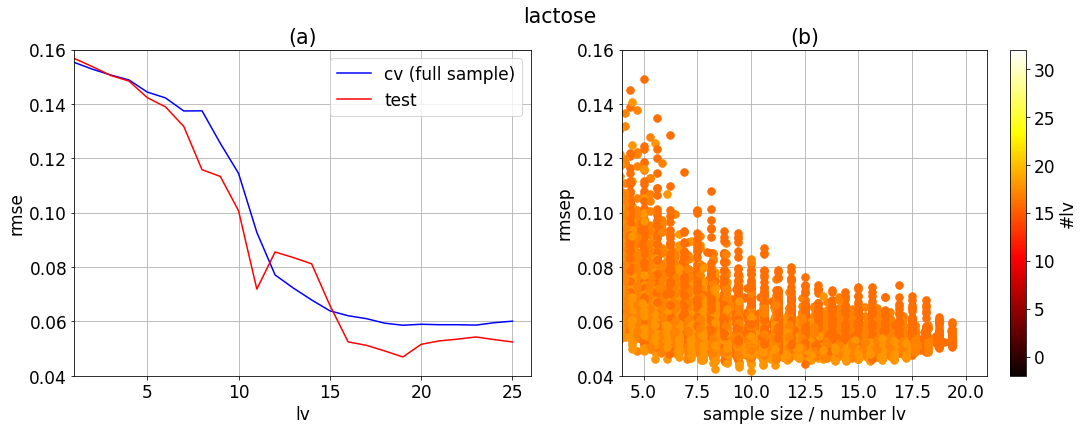
\includegraphics[width=0.8\textwidth]{manuscript/figures/d01_milk_general_framework.png}
\centering
\caption{(a) RMSECV based on the original set and RMSEP for Milk data set. (b) RMSEP values as function of the ratio $n/d$ gathering the results for $d$ = 16, 17 and 18.}
\label{fig_d01_milk_general_framework}
\end{figure}

\begin{figure}[b]
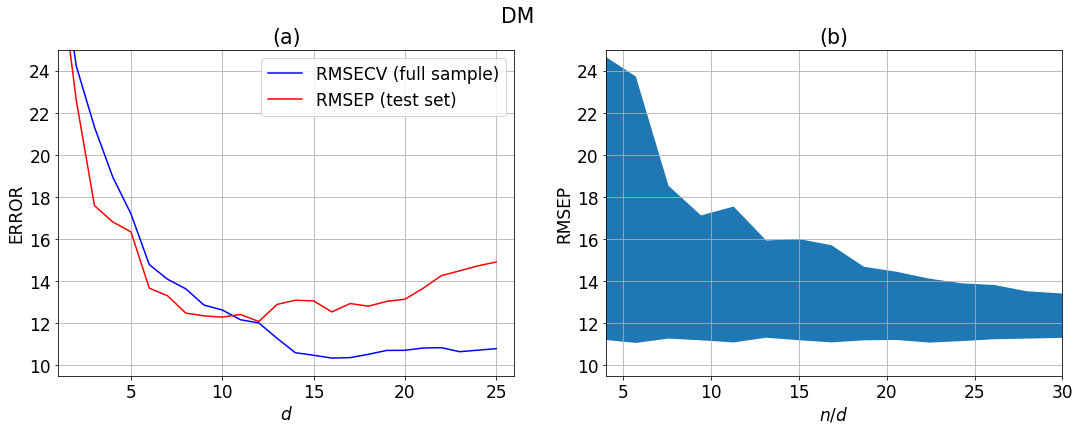
\includegraphics[width=0.8\textwidth]{manuscript/figures/d02_manure_general_framework.png}
\centering
\caption{(a) RMSECV based on the original set and RMSEP for Manure data set. (b) RMSEP values as function of the ratio $n/d$ gathering the results for $d$ = 11, 12, 13 and 14}
\label{fig_d02_manure_general_framework}
\end{figure}

\subsection*{Specific framework}\label{results:specframework}

\emph{What is the equivalence achieved between $\mathbf{S}_N$ and $\mathbf{S}_n$ by selection methods, input dimensionality and sample size?} 

Due to the vast quantity of results, the degree of equivalence between $\mathbf{S}_N$ and $\mathbf{S}_n$ is presented here for the different selection methods, sample sizes and a few values of the input dimensionality $a$. The impact of the entire range of $a$ for model performance is presented in the next section. Figure \ref{fig_specific_framework_detereigevect} shows the comparison of the eigenvectors of $\mathbf{S}_N$ and $\mathbf{S}_n$ for both of the case studies when the sample selection was made with $a=15$, 20 and 25 with each method. 

Across the different methods, the behavior of the determinant at a fixed $a$ was noticeably related to the sample size, yet differently for the different selection methods. Excluding DUP, all the other methods in both case studies showed similar results for $a=15$ and 20. Determinants above 0.8 were achieved with sample sizes below 30\% of N. When setting $a=25$ large differences were observed by the selected calibration sets across the different methods and sample sizes. In both case studies, CL and D-OPT selection showed a jump in the determinant around the same sample sizes. In the Manure case, KS related to CL and D-OPT in this behavior while it was PUCH in the Milk case. As expected, due to the nature of selection with DUP, the determinant presents a declination after crossing 50\% of the samples for selection. However, this decline was obtained for $a=20, 25$ and not for $a=15$ making evident the effect of the input dimensionality. RAND selection did not achieve a clear stabilization of the determinant compared to that of the other selection methods.

For KS, PUCH, CL and D-OPT, the stabilization of the determinant for $a=25$ at a value of $n$ was in line with the threshold found with the ratio $n/d>12$. The comparison of the resulting individual eigenvalues is therefore presented for the selection made with $a = 25$ for both case studies in Figures \ref{fig_d01_milk_specific_framework_eigenvalsratio} and \ref{fig_d02_manure_specific_framework_eigenvalsratio}. Each curve represents the eigenvalues ratio for a given value of $n$. With the exception of DUP selection, there is a clear convergence towards 1 of these ratios as $n$ increases. This suggests that, ideally, a subset of samples could be selected such that the resulting eigenvalues are uniformly close to the eigenvalues based on the total number of samples. For small sample sizes, a high variation of the ratios occurred revealing that even when selecting the samples with $a=25$, not all dimensions are equally represented in the subset. Most interestingly, high peaks and drops happened at the same dimensions indistinctly of the selection method. As $n$ increases, the curves are flatter indicating an equitable representation of the individual dimensions. 

In this comparison, the 50\% effect of DUP selection was detected as the ratio of the eigenvalues went under 1 after such a sample size $n$. In both case studies, KS, D-OPT and PUCH selection showed that there is generally no underestimation of variability as the eigenvalues ratio stayed above 1 with very few exceptions. No systematic behavior in the variability by eigenvalues was revealed by RAND selection. 

As CL is a more robust method compared to the other methods in terms of control over possible outliers, the eigenvalues ratio is overall more stable and closer to 1 in comparison with the other methods. In the Milk case, for very small sample sizes, some dimensions resulted in ratios between 0.5 and 1. D-OPT showed more linearity for the eigenvalues ratio as a function of the sample size compared to the other methods in both case studies. 

The possible risk of the non-uniform spanning of variability across the different dimensions was supported by the correlations between PC dimensions and the chemical constituent. Table \ref{tab_correlations} shows the Pearson correlations for both case studies. In the case of the Milk data set, PC's 18 and 21 showed higher correlations with lactose than even PC's 1 and 2. In the Manure case, DM had a higher correlation with PC 5 than PC 1, but the first 10 PC's accounted for the highest correlations. The impact of diminishing or underestimating the variability at certain dimensions is to be presented with respect to the PLSR model performance. In regard to the equivalence between $\mathbf{S}_N$ and $\mathbf{S}_n$, the degree of equivalence depended on the rank value of $a$ and a more uniform span of variability according to the eigenvalues could be obtained in both case studies with sample sizes according to $n/d>12$.  

\begin{table*}[t]
\centering
\begin{tabular}{|cc|cc|} 
\hline
\multicolumn{2}{|c|}{Milk (lactose)} & \multicolumn{2}{|c|}{Manure (DM)}\\
\hline
pc	& correlation	&  pc & correlation	\\
\hline
  1 & -0.1337 & 1 & -0.3132 \\
  2 & -0.1839 & 2 & -0.6231 \\
  3 & -0.0239 & 3 & -0.1587 \\
  4 &  0.2380 & 4 &  0.2220 \\
  5 &  0.0496 & 5 &  0.4036 \\
 16 &  0.0060 & 6 &  0.0299 \\
 17 &  0.0266 & 7 & -0.3102 \\
 18 &  0.4208 & 8 & 0.0521 \\
 19 &  0.1202 & 9 & 0.1543 \\
 20 &  0.0759 & 10& 0.0259 \\
 21 &  0.3819 &  & \\
 \hline
\end{tabular}
\caption{Pearson correlations between PC's and chemical component based on the selection set}
\label{tab_correlations}
\end{table*}


\begin{figure*}[t]
    \centering
    \subfigure[Milk]{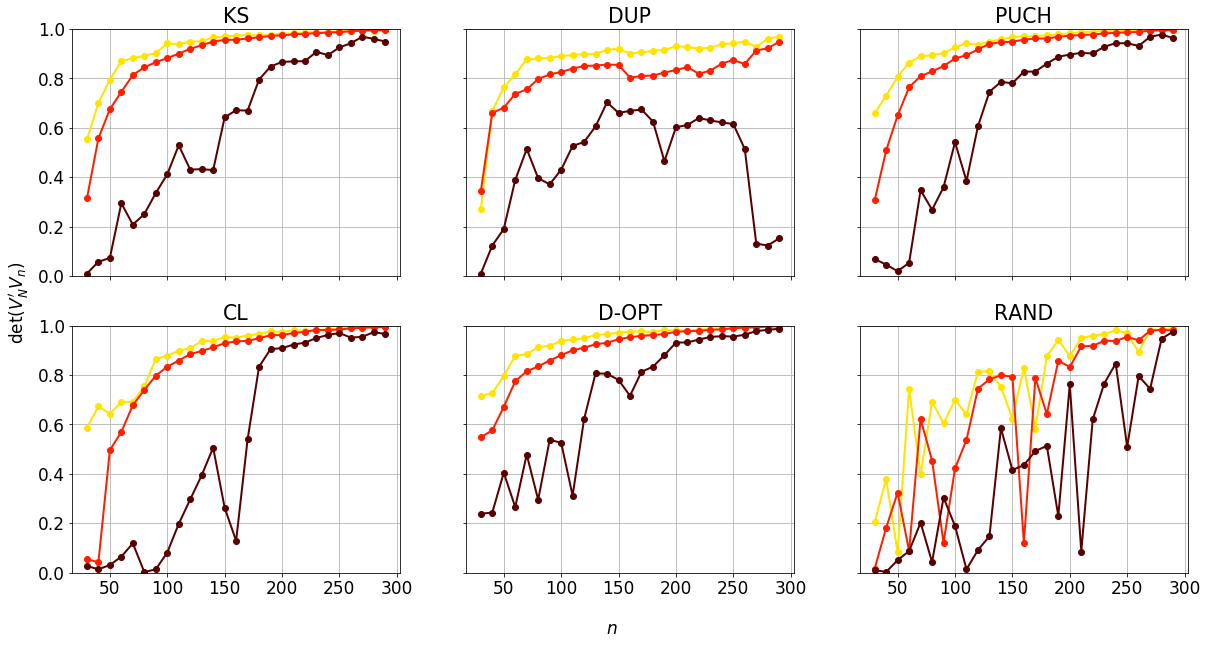
\includegraphics[width=0.6\textwidth]{manuscript/figures/d01_milk_specific_framework_detereigevect.png}} 
    \subfigure[Manure]{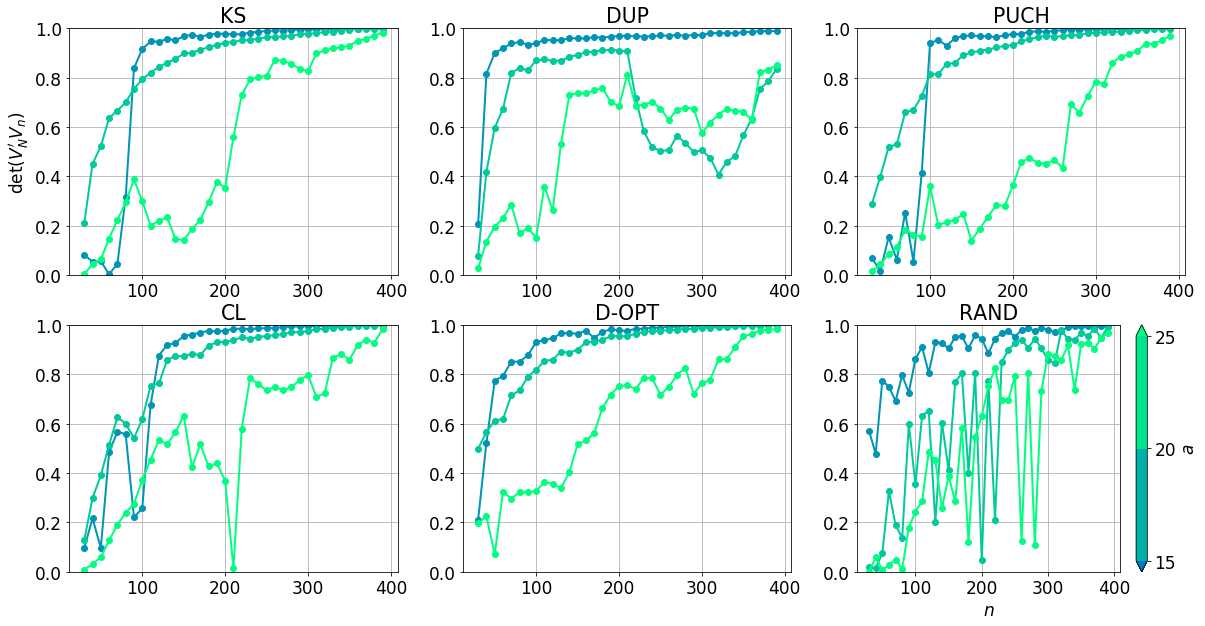
\includegraphics[width=0.6\textwidth]{manuscript/figures/d02_manure_specific_framework_detereigevect.png}}
    \caption{Comparison of eigenvectors when selecting samples with every method and input dimensionality $a=15,20,25$.}
    \label{fig_specific_framework_detereigevect}
\end{figure*}

\begin{figure}[b]
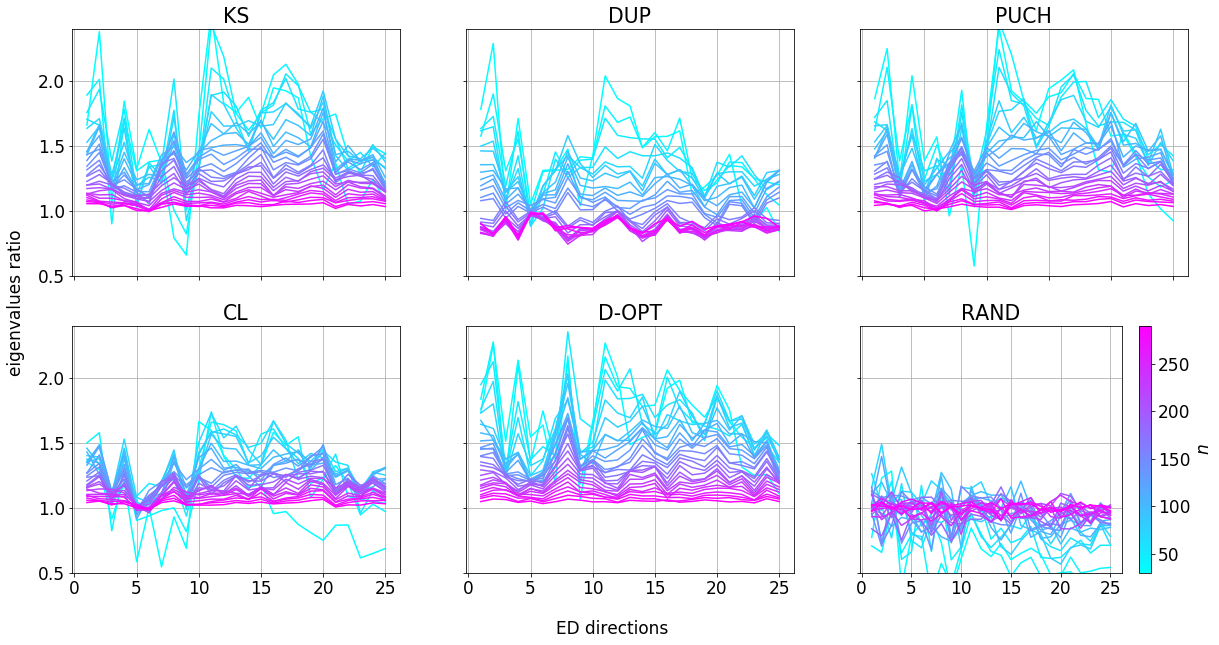
\includegraphics[width=0.8\textwidth]{manuscript/figures/d01_milk_specific_framework_eigenvalsratio.png}
\centering
\caption{Comparison of eigenvalues for Milk when selecting samples with every method and input dimensionality $a=25$.}
\label{fig_d01_milk_specific_framework_eigenvalsratio}
\end{figure}

\begin{figure}[b]
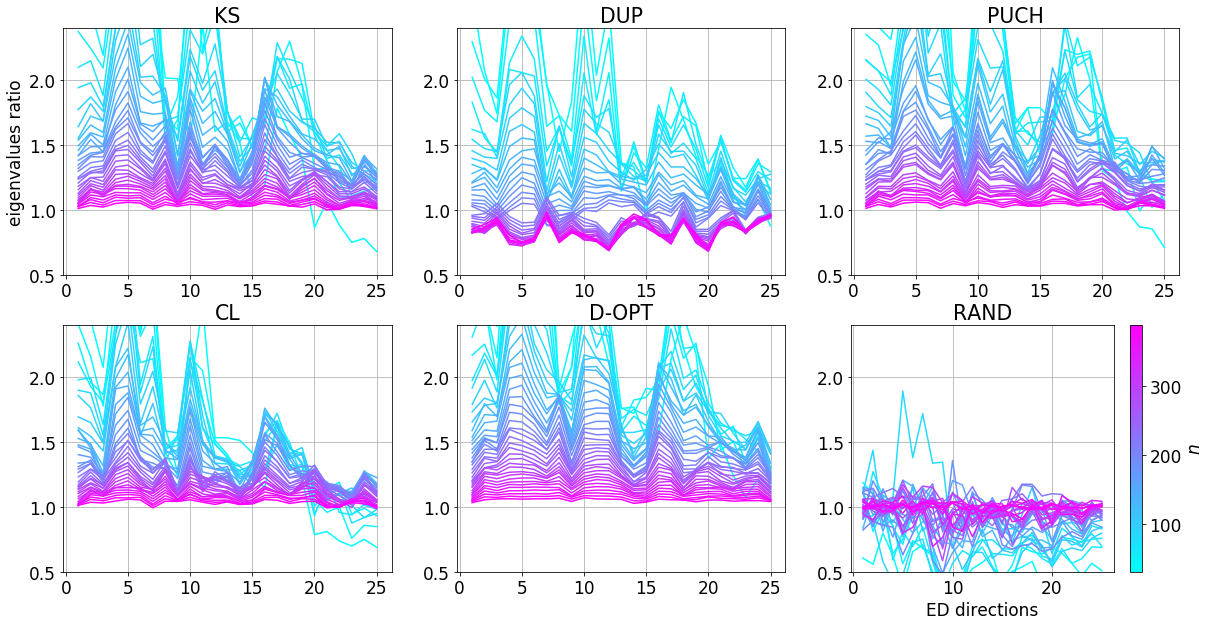
\includegraphics[width=0.8\textwidth]{manuscript/figures/d02_manure_specific_framework_eigenvalsratio.png}
\centering
\caption{Comparison of eigenvalues for Manure when selecting samples with every method and input dimensionality $a=25$.}
\label{fig_d02_manure_specific_framework_eigenvalsratio}
\end{figure}

\subsection*{Model performance}\label{results:modperformance}


\emph{What are the most optimal conditions of the three factors for satisfactory PLSR models?}

The simultaneous effect of the three selection factors on the performance of PLSR models was analyzed by comparing the RMSEP curves in each case study. The grid in Figures \ref{fig_d01_milk_model_performance} and \ref{fig_d02_manure_model_performance} shows the PLSR model performance for the Milk and the Manure case study, respectively. The selection methods are accommodated row-wise, punctual sample sizes are positioned column-wise and the color of the curves stands for the input dimensionality. The main insight when comparing both case studies in terms of the impact of the sample selection factors is that the stabilization or convergence of model performance occurred at the thresholds found for $n$ at the optimal complexity $d$. 

\begin{figure}[b]
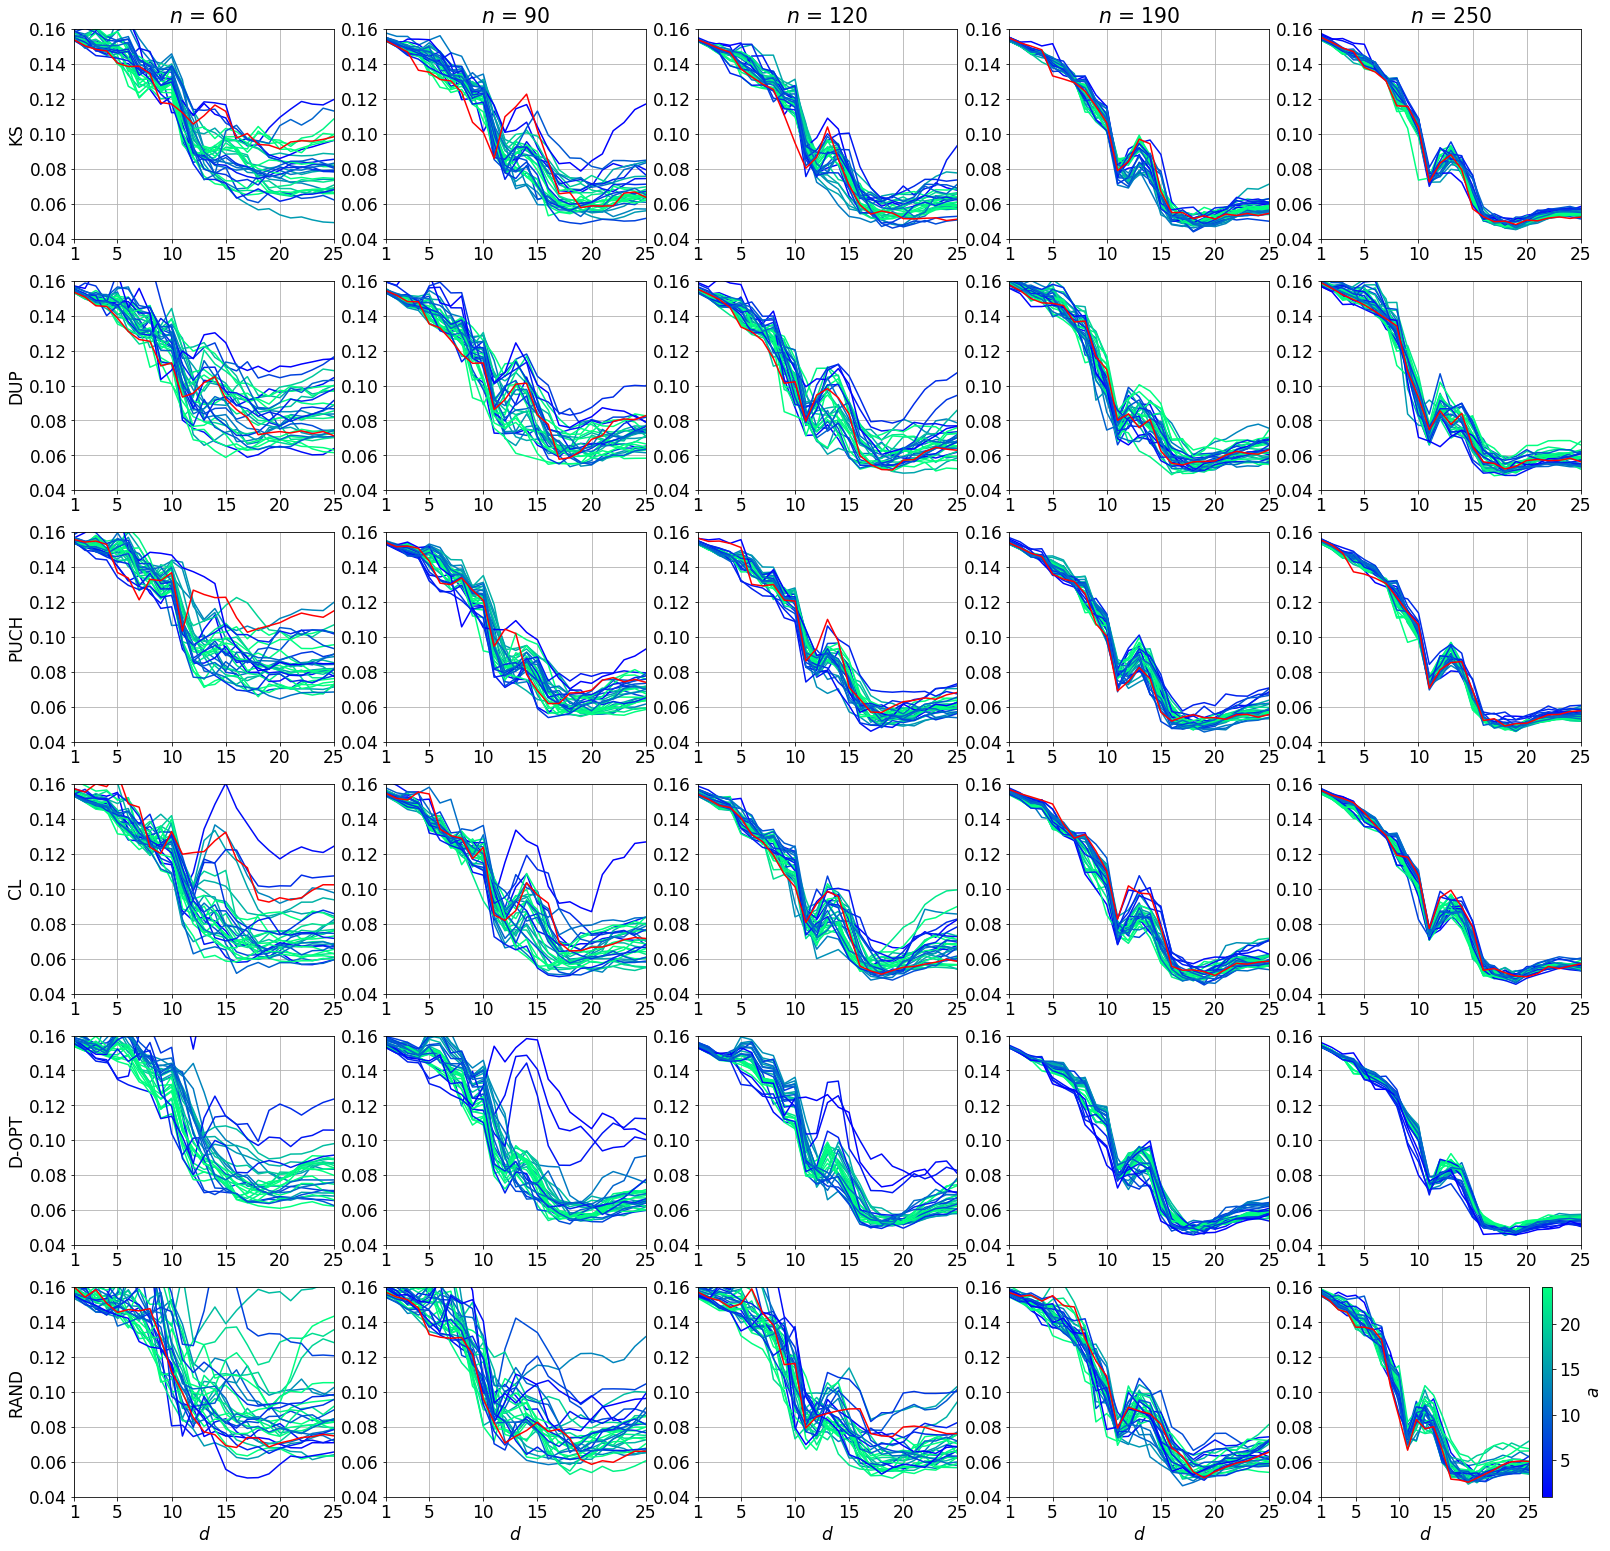
\includegraphics[width=0.8\textwidth]{manuscript/figures/d01_milk_model_performance.png}
\centering
\caption{Model performance to predict lactose according to selection method, input dimensionality and sample size. The red line represents input dimensionality $a=p$.}
\label{fig_d01_milk_model_performance}
\end{figure}

In both case studies, RAND selection resulted in higher performance uncertainty as the sample size decreased. For higher sample sizes surpassing the thresholds found in the general framework, RAND selection rendered calibration sets that were equally optimal as the sets delivered by any other selection method. In the prediction of lactose, the model performance for the selected sets of size $n=60$ was highly uncertain and no clear relation was found between a satisfactory performance and the selection method or the input dimensionality. Nonetheless, for such a small $n$, the selected set by D-OPT with a high value of $a$ produced consistently models with better performance. The same result was detected for D-OPT for other small sample sizes ($n=90$ and $n=120$). This differentiation of the effect of the input dimensionality was not equally clear for small sample sizes with the other methods. Moreover, when selecting samples based on the original $\mathbf{X}$ matrix (i.e. $a=p$), there was no satisfactory result for the small sample sizes compared to values of $a$ between 15 and 25. When surpassing the threshold and selecting more than 160 samples, the performance of the models with the different methods and input dimensionality stabilized and no important or systematic difference was observed.

The model performance for the Manure case suggested similar conclusions on the effect of the factors as in the Milk case study. In particular, for a small sample size as $n=60$, D-OPT selection showed a more stable performance around $d = 11$ for large values of $a$ than the performance stability by the other methods. This stabilization by D-OPT was observed more clearly for $n=90$ from 8 to 16 latent variables. Once the threshold $n/d>12$ was surpassed, which happened between 130 and 140 samples, all the selection methods except DUP with $a$ between 20 and 25 rendered calibration sets with satisfactory performance. RAND selection also proved here to render similar results as other selection methods as the sample size increased. 




\begin{figure}[b]
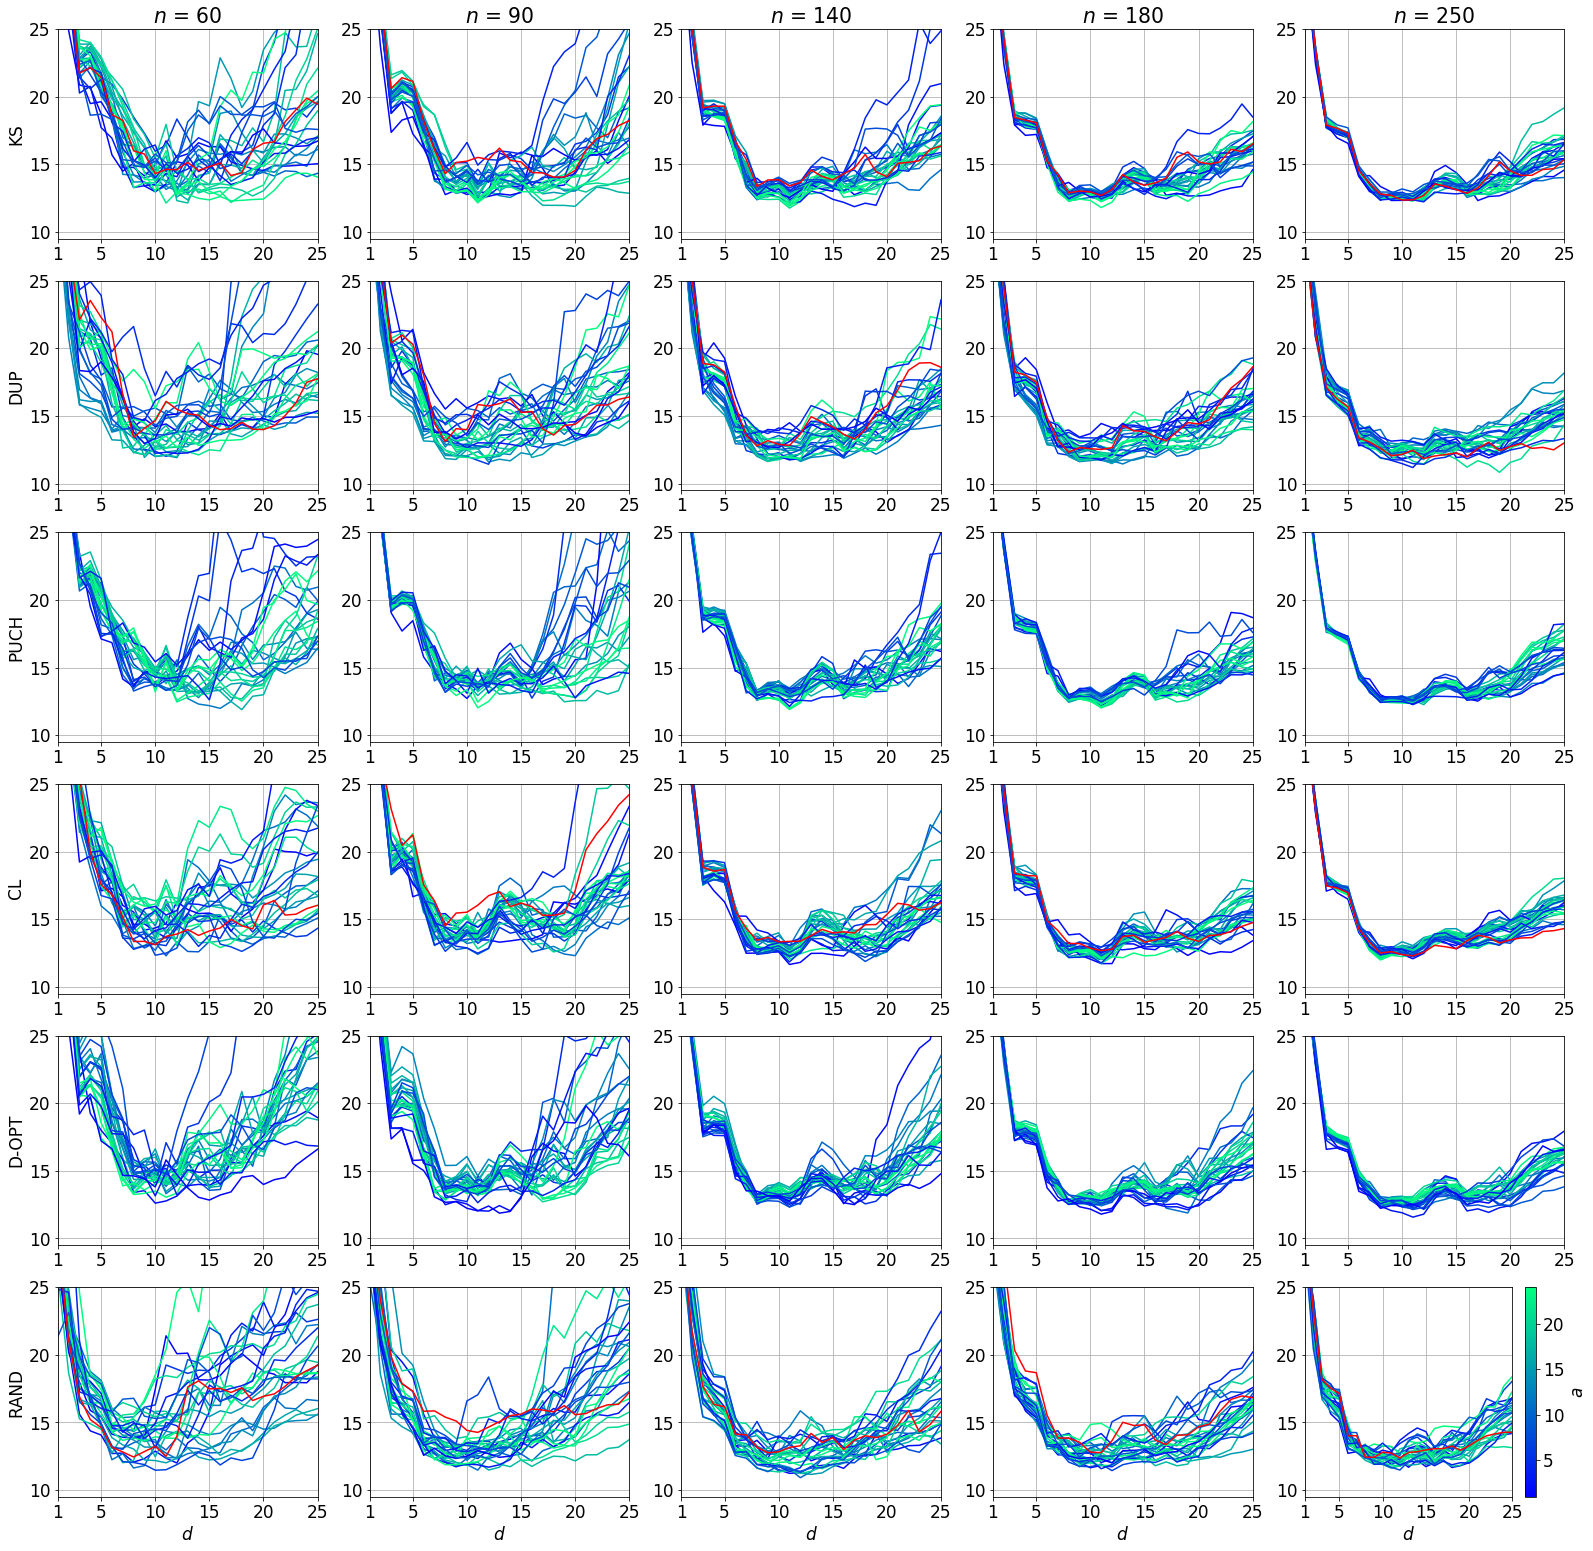
\includegraphics[width=0.8\textwidth]{manuscript/figures/d02_manure_model_performance.png}
\centering
\caption{Model performance to predict DM according to selection method, input dimensionality and sample size. The red line represents input dimensionality $a=p$.}
\label{fig_d02_manure_model_performance}
\end{figure}

% -----------------------------------------------------
% ------------------- discussion  ------------
% -----------------------------------------------------



\section*{Discussion}\label{discussion}

When positioning the PLSR algorithm in the general framework of statistical learning theory, it was found that indeed, the sample size to be considered for multivariate calibration models cannot be thought outside the $VC$ dimension (i.e. model complexity). This means that a sample size $n$ will be differently optimal for an easy-to-predict chemical constituent than for another one that is harder to predict. This was revealed by the analysis of the ratio $n/d$ and the optimal sample sizes obtained in each case study. The level of easiness to predict is what the $VC$ dimension or model complexity represents. It was confirmed that a ratio $n/d>20$ accounts for a sample size that is rather large for a satisfactory calibration model. Based on the results of the present study, for which a hard-to-predict component (lactose) and an easier component (DM) were analyzed, evidence was obtained that a satisfactory calibration model can be built with $n/d>12$. Although in practice the problem of unsupervised sample selection is encountered when there is no data available for the target variable $y$, it is possible to make an estimation of $d$ based on the literature and expertise of the problem at hand.

In Au (2020)\cite{Au2020}, thresholds for the optimal sample size were found in absolute numbers. However, as the sample size steps taken were large, the detected thresholds corresponded to sample sizes for which the ratio $n/d>20$, as the optimal model complexity shown there was about 7 to 10 latent variables. Those results still confirm the theory based on the $n/d$ given by Vapnik \cite{Vapnik2000}.

The leading feature to address the current problem is that of spanning as much as possible the variability contained in the available selection set so that a representative subset of samples is obtained. In the context of chemometrics, this feature has not been concretely translated into a mathematical criterion, which at the same time is to be defined based on the model architecture that best describes the relationship between $\mathbf{X}$ and $y$. The specific framework analysis shows the role that the matrix $\mathbf{S}$ plays in the PLSR model, making it the mathematical element that can be controlled in an unsupervised setting. Therefore, finding a subset of $n$ samples that renders $\mathbf{S}_n$ equivalent to $\mathbf{S}_N$ is a proposed definition about the representativity of the selected samples. 

The results about the comparison of eigenvectors and eigenvalues showed that, provided the input dimensionality of $\mathbf{S}$, there is convergence in the equivalence of these matrices. In practice, if the number of samples can be decided based on ratio $n/d$, a suitable value for $a$ and the samples that render equivalent $\mathbf{S}_n$ and $\mathbf{S}_N$ can be detected by evaluating the determinant and eigenvalues ratio criteria. Based on the model performance results when selecting samples with a low input dimensionality, it was detected that keeping dimensions of low variability out of the sample selection strategy may greatly compromise the performance of the model after gathering reference analyses. This insight was supported by the model performance achieved with high values of $a$ at least for KS, CL, PUCH and D-OPT and the high correlations between PC dimensions of low variability and $y$ in both case studies. In the works that are found in the literature of chemometrics applications, the unsupervised sample selection has been applied with different methods and a reduced input dimensionality, but no analysis is generally found on the effect of the latter factor \cite{Naes1990, Brandmaier2012, Nawar2018, Au2020}. Complementary, it is not conclusive that selecting the samples with the original dimensionality of $\mathbf{X}$ was particularly advantageous than reducing it to $a<<p$. This is particularly relevant because D-OPT does not support the original matrix $\mathbf{X}$ when its rank is deficient.

The effect of the selection method is largely diminished once the sample size and the dimensionality $a$ are controlled. Nonetheless, each of the selection methods operates under their own criterion to span the variability. DUP is the least suitable method for unsupervised sample selection as it is concretely designed to separate the set in exactly 50\% parts. It functions by finding two replicate submatrices in the matrix $\mathbf{X}$, which might not be the ideal separation according to the threshold for the optimal sample size as confirmed by the presented results. D-OPT selection, on the other hand, proved to deliver an optimal selection consistently for high values of $a$. This method, however, is characterized by overestimating the variability, representing a possible challenge in presence of bad outliers or an advantage for good leverage points. CL demonstrates to be the most robust strategy for sample selection although it represents a risk when the sample size $n$ does not correspond to $n$ well-defined groups existing in the original set. This insight was hypothesized based on the drop of the determinant rendered by CL in both case studies. Together with KS and PUCH selection, representative calibration sets can be delivered by these methods, but the results on model performance showed that this aspect is highly dependent on punctual values of the dimensionality $a$, rather than ranges of it. Therefore, a suitable criterion would then be one that, provided a rank $a$, delivers a set for which $\mathbf{S}_n$ and $\mathbf{S}_N$ are equivalent in terms of their eigenvectors and eigenvalues, subject to a ratio of the eigenvalues above 1 and as uniform as possible across the SVD directions.

An important feature that is of question when using D-OPT selection is the so-called \emph{effects} to include, concretely, the polynomial degree of the input variables \cite{Goos2011}. When including only the main effects, D-OPT unavoidably selects the outer layer of the data variability. For particular purposes of the theory and applications of Experimental Design, interactions and higher order effects are commonly considered for sample selection \cite{Brandmaier2012}. However, in multivariate calibration and unsupervised sample selection, the absence of prior information does not justify the inclusion of other types of effects based on the model architecture of the PLSR model. Including high order effects is a practical strategy to select more central points, but there is no theoretical support for it in the context of the present work.

A final additional aspect comes about preprocessing. Several authors still consider specific preprocessing techniques to filter out certain spectral attributes from the signals. For sample selection, previous work was found commenting on the possible advantages of preprocessing the spectral data for unsupervised sample selection \cite{Liu2019}. However, initial experiments in the current case studies suggested that assuming advanced preprocessing such as scattering correction resulted in sets rendering calibration models with poor performance. Therefore, strong assumptions on preprocessing prior to obtaining reference analyses may not be advantageous.


% -----------------------------------------------------
% ------------------- a scheme  ------------
% -----------------------------------------------------

\section*{A scheme for sample selection}\label{scheme}

Following the exhaustive comparison of the factors involved into unsupervised sample selection, a scheme is defined to approach the current challenge in NIR applications and multivariate calibration. Optimal sample sizes can be calculated based on the threshold $n/d>12$. A maximum value for the PLSR model complexity $d$ can be established based on literature. Once $n$ is calculated, a value for the input dimensionality $a$ can be found by evaluating at what value of $a$ there is convergence in equivalence between $\mathbf{S}_N$ and $\mathbf{S}_n$. This ensures that the dimensions included in the selection account for PC's of small variability that can be beneficial for the PLSR model if a hard-to-predict constituent is involved. The samples can be selected with KS, PUCH, CL or D-OPT as they proved to deliver calibration sets for satisfactory models after controlling $n$ and $a$. D-OPT proved to have better consistency when the sample size is strictly restricted to the minimum value according to the thresholds. 


% -----------------------------------------------------
% ------------------- conclusions  ------------
% -----------------------------------------------------

\section*{Conclusions}\label{conclusions}

The proposed scheme was developed in the context of PLSR models. However, most model architectures, including nonlinear models such as neural networks or support vector machines relate to a $VC$ dimension which can be theoretically determined or practically estimated \cite{Vapnik2019, Vapnik1994}. This is also not restricted only to regression models, the same ideas apply for classification models. This means that optimal sample sizes can be calculated based on the ratio $n/d$ if an estimation on the model complexity $d$ can be found for the problem at hand. 

The criterion based on the equivalence between $\mathbf{S}_N$ and $\mathbf{S}_n$ is specific for the PLSR model architecture or similar models such as PLS discriminant analysis, linear regression, among others. For every model architecture, it is advisable to identify the mathematical components that could be controlled in unsupervised sample selection \cite{Li2020}.  




% -----------------------------------------------------
% ------------------- data availability  ------------
% -----------------------------------------------------

\section{Data availability}

All the methodology that was used in the present work is available for public share. 

% -----------------------------------------------------
% ------------------- acknowledgements  ------------
% -----------------------------------------------------

\begin{acknowledgement}

Valeria Fonseca Diaz is funded as aspirant to doctoral fellow of
the Research Foundation-Flanders (FWO Brussels, Belgium).
The authors thank Dr. Raffaele Vitale and professor Peter Goos (KU Leuven, Belgium) for their suggestions on the conducted analysis given their expertise in Chemometrics and Experimental Design. 
\end{acknowledgement}

% -----------------------------------------------------
% ------------------- bibliography  ------------
% -----------------------------------------------------



\bibliography{biblio}


\end{document}

